
Standard unsupervised methods for dependency detection, such as the
canonical correlation analysis or the symmetric information bottleneck,
seek maximal dependency between two data sets with minimal assumptions
about the dependencies. The unconstrained models involve high degrees
of freedom when applied to high-dimensional genomic observations. Such
flexibility can easily lead to overfitting, which is even worse for
more flexible nonparametric or nonlinear, kernel-based dependency
discovery methods.  Several ways to regularize the solution have been
suggested to overcome associated problems, for instance by imposing
sparsity constraints on the solution space \citep{Bie03, Vinod76}.

In many applications prior information of the dependencies is
available, or particular types of dependency are relevant for the
analysis task. Such prior information can be used to reduce the
degrees of freedom in the model, and to regularize dependency
detection. In the cancer gene discovery application of
Publication~\ref{MLSP}, DNA mutations are systematically correlated
with transcriptional activity of the genes within the affected region,
and identification of such regions is a biomedically relevant research
task. Prior knowledge of chromosomal distances between the
observations can improve the detection of the relevant spatial
dependencies. However, principled approaches to incorporate such prior
information in dependency modeling have been
missing. Publication~\ref{MLSP} introduces regularized models for
dependency detection based on classical canonical correlation analysis
\citep{Hotelling36} and its probabilistic formulation
\citep{Bach05}. The models are extended by incorporating appropriate
prior terms, which are then used to reduce the degrees of freedom
based on prior biological knowledge.


\subsubsection{Correlation-based variant}

In order to introduce the regularized dependency detection framework
of Publication~\ref{MLSP}, let us start by considering regularization
of the classical correlation-based CCA. This searches for arbitrary
linear projection vectors \(\vx, \vy\) that maximize the correlation
between the projections of the data sets \(\X, \Y\). Multiple
projection components can be obtained iteratively, by finding the most
correlating projection first, and then consecutively the next ones
after removing the dependencies explained by the previous CCA
components. The procedure will identify maximally dependent linear
subspaces of the investigated data sets. To regularize the solution,
Publication~\ref{MLSP} couples the projections through a
transformation matrix \(\T\) in such a way that \(\vy = \T \vx\). With
a completely unconstrained \(\T\) the model reduces to the classical
unconstrained CCA; suitable constraints on can be used to regularize
dependency detection.

To enforce regularization one could for instance prefer solutions for
\(\T\) that are close to a given transformation matrix, \(\T \sim
\M\), or impose more general constraints on the structure of the
transformation matrix that would prefer particular rotational or other
linear relationships. Suitable constraints depend on the particular
applications; the solutions can be made to prefer particular types of
dependency in a soft manner by appropriate penalty terms. In
Publication~\ref{MLSP} the completely unconstrained CCA model has been
compared with a fully regularized model with \(\T = \I\); this encodes
the biological assumption that probes with small chromosomal distances
tend to capture more similar signal between gene expression and copy
number measurements than probes with a larger chromosomal distance;
the projection vectors characterize this relationship, and are
therefore expected to have similar form, \(\vx \sim \vy\). Utilization
of other, more general constraints in related data integration tasks
provides a promising topic for future studies.

The correlation-based treatment provides an intuitive and easily
implementable formulation for regularized dependency
detection. However, it lacks an explicit model for the shared and
data-specific effects, and it is likely that some of the
dataset-specific effects are captured by the correlation-maximizing
projections. This is suboptimal for characterizing the shared effects,
and motivates the probabilistic treatment.

\subsubsection{Probabilistic dependency detection with similarity constraints}

The probabilistic approach for regularized dependency detection in
Publication~\ref{MLSP} is based on an explicit model of the
data-generating process formulated in Equation~(\ref{eq:genmodel}). In
this model, the transformation matrices \(\W_x\), \(\W_y\) specify how
the shared latent variable \(\Z\) is manifested in each data set
\(\X\), \(\Y\), respectively. In the standard model, the relationship
between the transformation matrices is not constrained, and the
algorithm searches for arbitrary linear transformations that maximize
the likelihood of the observations in
Equation~(\ref{eq:ccalikelihood}). The probabilistic formulation opens
up possibilities to guide dependency search through Bayesian priors.

In Publication~\ref{MLSP}, the standard probabilistic CCA model is
extended by incorporating additional prior terms that regularize the
relationship by reparameterizing the transformation matrices as \(\W_y
= \T\W_x\), and setting a prior on \(\T\). The treatment is analogous
to the correlation-based variant, but now the transformation matrices
operate on the latent components, rather than the observations. This
allows to distinguish the shared and dataset-specific effects more
explicitly in the model. The task is then to learn the optimal
parameter matrix \(\W = [\Wx; \Wy]\), given the constraint \(\W_y =
\T\W_x\). The Bayes' rule gives the model likelihood

\begin{equation}\label{eq:ccafull}
  p(\X, \Y, \W, \Psib) \sim p(\X, \Y | \W, \Psib) p(\W, \Psib).
\end{equation}

\noindent The likelihood term \(p(\X, \Y | \W, \Psib)\) can be
calculated based on the model in Equation~(\ref{eq:genmodel}). This
defines the objective function for standard probabilistic CCA, which
implicitly assumes a flat prior \(p(\W, \Psib) \sim 1\) for the model
parameters. The formulation in Equation~(\ref{eq:ccafull}) makes the
choice of the prior explicit, allowing modifications on the prior
term. To obtain a tractable prior, let us assume that the prior
factorizes as \(p(\W, \Psib) = p( \W ) p( \Psib )\). The first term
can be further decomposed as \(p(\W) \sim p(\W_x) p(\T)\), assuming
independent priors for \(\W_x\) and \(\T\). A convenient and tractable
prior for \(\T\) is provided by the matrix normal
distribution:\footnote{\(\Nm(\T | \M, \U, \Vb) \sim
  exp\left(-\frac{1}{2} Tr\{\U^{-1}(\T-\M)\Vb^{-1}(\T -
    \M)^T\}\right)\) where \(\M\) is the mean matrix, and \(\U\) and
  \(\Vb\) denote row and column covariances, respectively.}

\begin{equation}\label{eq:Nm}
  p(\T) = \Nm(\T | \M, \U, \Vb).
\end{equation}

\noindent For computational simplicity, let us assume independent rows
and columns with \(\U = \Vb = \sigma_T \I\). The mean matrix \(\M\)
can be used to emphasize certain types of dependency between \(\Wx\)
and \(\Wy\). Assuming uninformative, flat priors \(p(\Wx) \sim 1\) and
\(p(\Psib) \sim 1\), as in the standard probabilistic CCA model, and
denoting \(\bSigma = \W\W^T + \Psib \), the negative log-likelihood of
the model is

\begin{equation}\label{eq:simccacost}
  -logp(\X, \Y, \W, \Psib) \sim log|\bSigma| + Tr \bSigma^{-1} \tilde{\bSigma} +
  \frac{\parallel \T - \M \parallel_{F}^2}{2\sigt}.
\end{equation}

\noindent This is the objective function to minimize. Note that this
has the same form as the objective function of the standard
probabilistic CCA, except the additional penalty term
\(\frac{\parallel \T - \M \parallel_{F}^2}{2\sigt}\) arising from the
prior \(p(\T)\). This yields the cost function employed in
Publication~\ref{MLSP}. In our cancer gene discovery application the
choice \(\M = \I\) is used to encode the biological prior constrain
\(\T \approx \I\), which states that the observations with a small
chromosomal distance should on average show similar responses in the
integrated data sets, i.e., \(\Wx \approx \Wy\). The regularization
strength can be tuned with \(\sigt\). A fully regularized model is
obtained with \(\sigt \rightarrow 0\). When \(\sigt \rightarrow
\infty\), $\W_x$ and $\W_y$ become independent {\it a priori},
yielding the ordinary probabilistic CCA. The \(\sigt\) can be used to
regularize the solution between these two extremes. Note that it is
possible to incorporate also other types of prior information
concerning the dependencies into the model through \(p(\T)\).

The model parameters \(\W\), \(\Psib\) are estimated with the EM
algorithm. The regularized version is not analytically tractable with
respect to \(\W\) in the general case, but can be optimized with
standard gradient-based optimization techniques. Special cases of the
model have analytical solutions, which can speed up the model fitting
procedure. In particular, the fully regularized and unconstrained
models, obtained with \(\sigt = 0\) and \(\sigt = \infty\)
respectively, have closed-form solutions for \(\W\). Note that the
current formulation assumes that the regularization parameters \(\M,
\sigt\) are defined prior to the analysis. Alternatively, these
parameters could be optimized based on external criteria, such as
cancer gene detection performance in our application, or learned from
the data in a fully Bayesian treatment these parameters would be
treated as latent variables. Incorporation of additional prior
information of the data set-specific effects through priors on
\(\W_x\) and \(\Psib\) provides promising lines for further work.

\subsection{Cancer gene discovery with dependency detection}

The regularized models provide a principled framework for studying
associations between transcriptional activity and other regulatory
layers of the genome. In Publication~\ref{MLSP}, the models are used
to investigate cancer mechanisms. DNA copy number changes are a key
mechanism for cancer, and integration of copy number information with
mRNA expression measurements can reveal functional effects of the
mutations. While causation may be difficult to grasp, study of the
dependencies can help to identify functionally active mutations, and
to provide candidate biomarkers with potential diagnostic, prognostic
and clinical impact in cancer studies.

The modeling task in the cancer gene discovery application of
Publication~\ref{MLSP} is to identify chromosomal regions that show
exceptionally high levels of dependency between gene copy number and
transcriptional levels.  The model is used to detect dependency within
local chromosomal regions that are then compared in order to identify
the exceptional regions. The dependency is quantified within a given
region by comparing the strength of shared and data set-specific
signal. High scores indicate regions where the shared signal is
particularly high relative to the data-set-specific effects.  A
sliding-window approach is used to screen the genome for
dependencies. The regions are defined by the \(d\) closest probes
around each gene. Then the dimensionality of the models stays
constant, which allows direct comparison of the dependency measures
between the regions without additional adjustment terms that would be
otherwise needed to compensate for differences in model complexity.

Prior information of the dependencies is used to regularize cancer
gene detection. Chromosomal gains and losses are likely to be
positively correlated with the expression levels of the affected genes
within the same chromosomal region or its close proximity; copy number
gain is likely to increase the expression of the associated genes
whereas deletion will block gene expression.  The prior information is
encoded in the model by setting \(\M = \I\) in the prior term
\(p(\T)\). This accounts for the expected positive correlations
between gene expression and copy number within the investigated
chromosomal region. Regularization based on such prior information is
shown to improve cancer gene detection performance in
Publication~\ref{MLSP}, where the regularized variants outperformed
the unconstrained models.

A genome-wide screen of 51 gastric cancer patients
\citep{Myllykangas08jc} reveals clear associations between DNA copy
number changes and transcriptional activity. The Figure~\ref{fig:17q}
illustrates dependency detection on chromosome arm 17q, where the
regularized model reveals high dependency between the two data sources
in a known cancer-associated region.  The regularized and
unconstrained models were compared in terms of receiver-operator
characteristics calculated by comparing the ordered gene list from the
dependency screen to an expert-curated list of known genes associated
with gastric cancer \citep{Myllykangas08jc}. A large proportion of the
most significant findings in the whole-genome analysis were known
cancer genes; the remaining findings with no known associations to
gastric cancer are promising candidates for further study.

Biomedical interpretation of the model parameters is also
straightforward. A ML estimate of the latent variable values \(\Z\)
characterizes the strength of the shared signal between DNA mutations
and transcriptional activity for each patient. This allows robust
identification of small, potentially unknown patient subgroups with
shared amplification effects. These would remain potentially
undetected when comparing patient groups defined based on existing
clinical annotations. The parameters in \(\W\) can downweigh signal
from poorly performing probes in each data set, or probes that measure
genes whose transcriptional levels are not functionally affected by
the copy number change. This provides tools to distinguish between
so-called {\it driver} mutations having functional effects from less
active {\it passenger} mutations, which is an important task in cancer
studies.  On the other hand, the model can combine statistical power
across the adjacent measurement probes, and it captures the strongest
shared signal in the two sets of observations. This is useful since
gene expression and copy number data are typically characterized by
high levels of biological and measurement variation and small sample
size.

\begin{figure}[ht!]
\centerline{
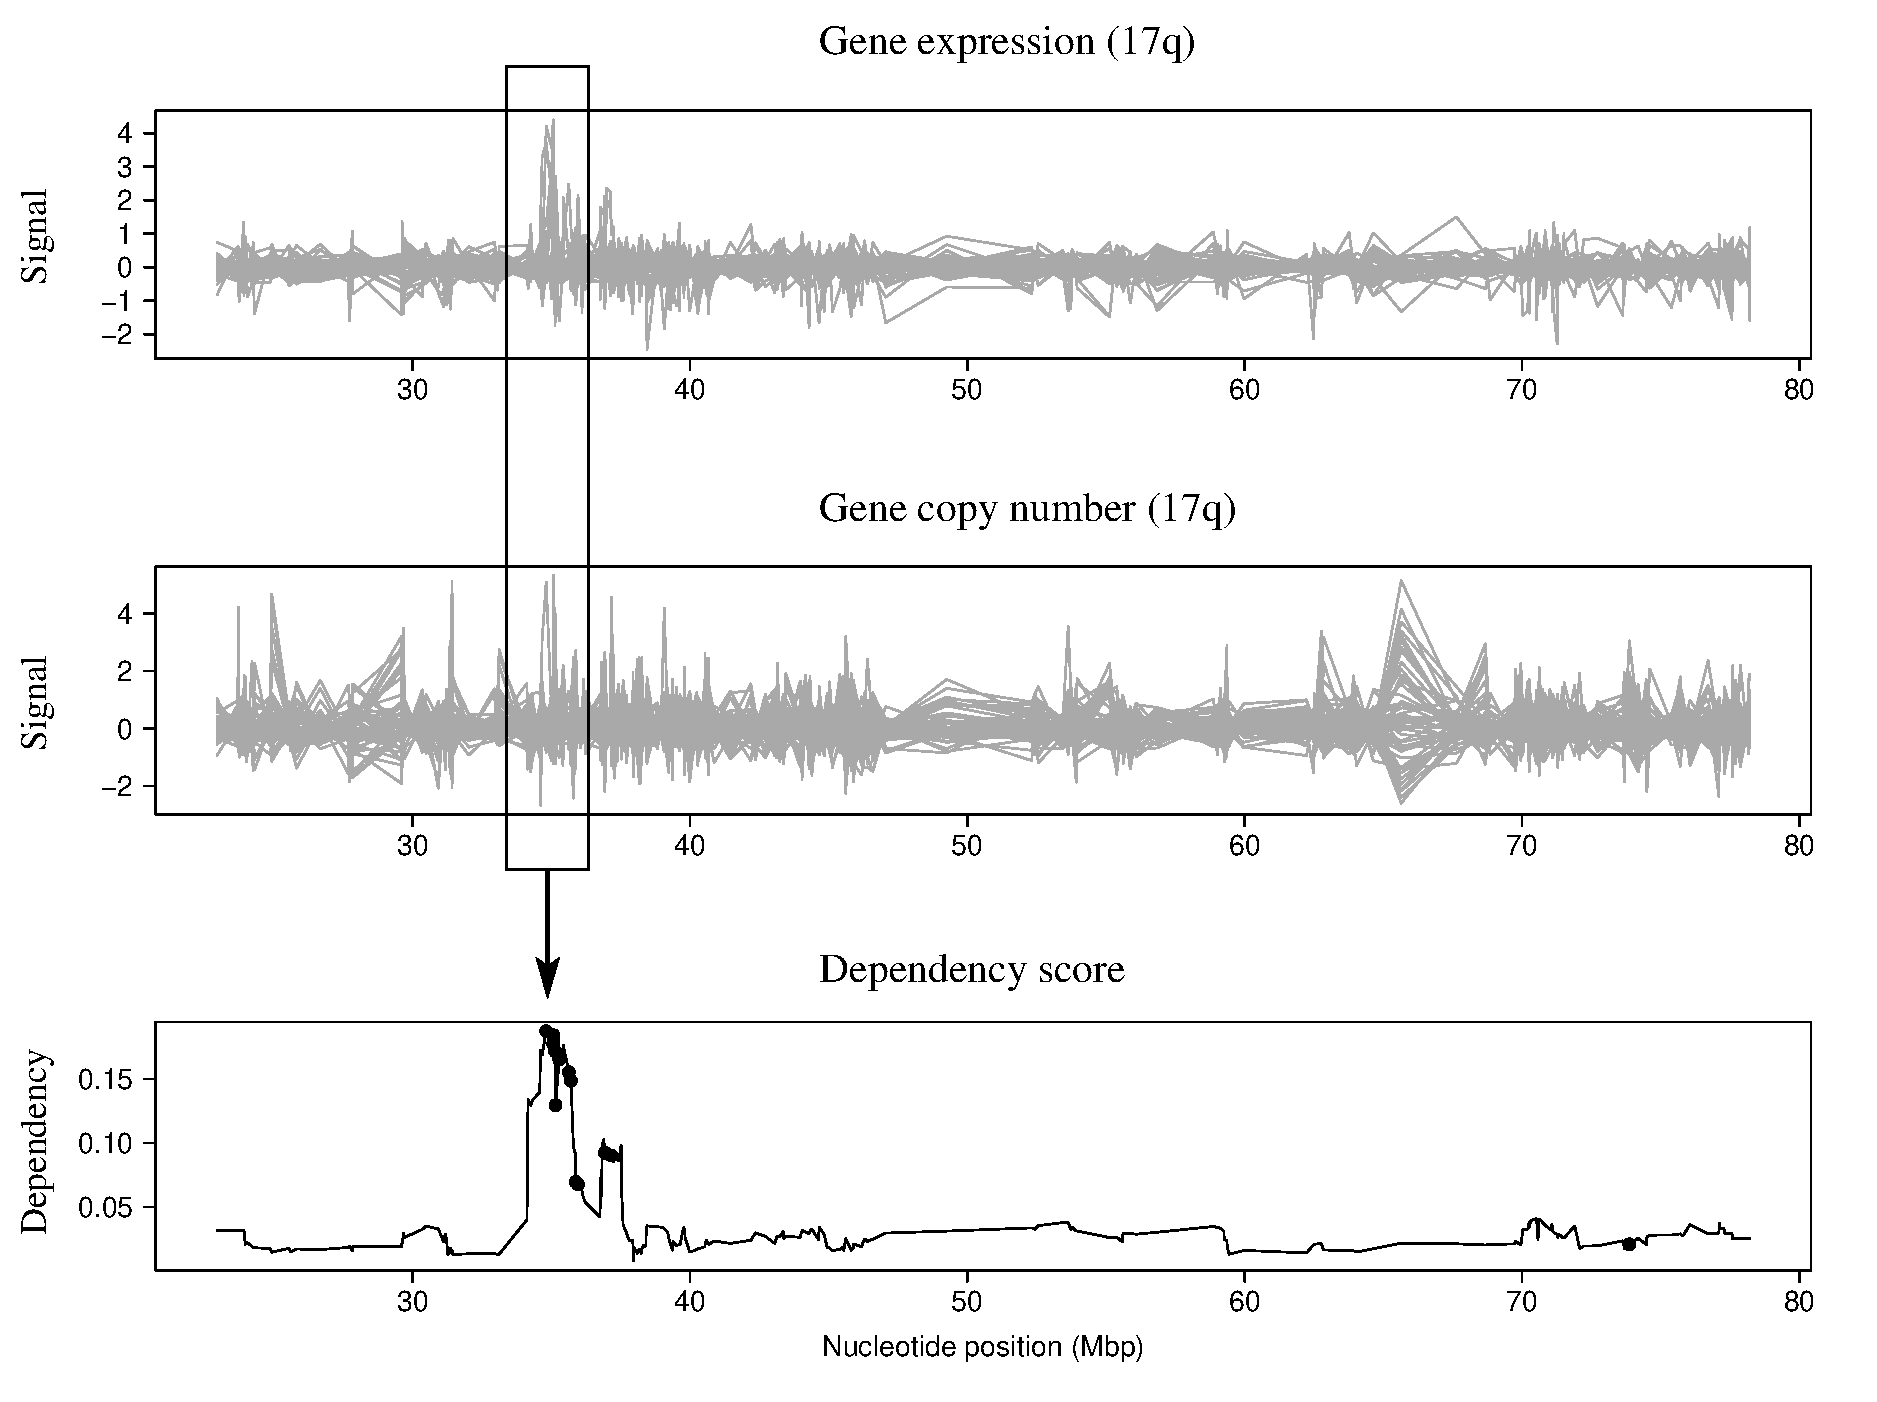
\includegraphics[width=1\textwidth]{pic/17q.eps}} 
\caption{Gene expression, copy number signal, and the dependency score
  along the chromosome arm 17q obtained with the regularized latent
  variable framework in Equation~\ref{eq:simccacost}. Known
  cancer-associated genes from an expert-curated list are marked with
  black dots.}
\label{fig:17q}
\end{figure}
% Produced with pic/chr17q.R + xfig

\subsubsection{Related approaches}

Integration of chromosomal aberrations and transcriptional activity is
an actively studied data integration task in functional genomics. The
first studies with standard statistical tests were carried out by
\citet{Hyman2002} and \citet{Phillips2001} when simultaneous
genome-wide observations of the two data sources had become available.
The modeling approaches utilized in this context can be roughly
classified in regression-based, correlation-based and latent variable
approaches. The regression-based models \citep{Adler2006, Bicciato09,
  Wieringen09} characterize alterations in gene expression levels
based on copy number observations with multivariate regression or
closely related models. The correlation-based approaches
\citep{Gonzalez2009, Schafer09, Soneson2010} provide symmetric models
for dependency detection, based on correlation and related statistical
models. Many of these methods also regularize the solutions, typically
based on sparsity constraints and non-negativity of the projections
\citep{LeCao2009, Waaijenborg2008, Witten09, Parkhomenko2009}. The
correlation-based approach in Publication~\ref{MLSP} introduces a
complementary approach for regularization that constrains the
relationship between subspaces where the correlations are
estimated. The latent variable models by \cite{Berger06, Shen09,
  Vaske2010}, and Publication~\ref{MLSP} are based on explicit
modeling assumptions concerning the data-generating processes. The
iCluster algorithm \citep{Shen09} is closely related to the latent
variable model considered in Publication~\ref{MLSP}. While our model
detects continuous dependencies, iCluster uses a discrete latent
variable to partition the samples into distinct subgroups.  The
iCluster model is regularized by sparsity constraints on \(\W\), while
we tune the relationship between \(\Wx\) and \(\Wy\). Moreover, the
model in Publication~\ref{MLSP} utilizes full covariance matrices to
model for the dataset-specific effects, whereas iCluster uses diagonal
covariances. The more detailed model for dataset-specific effects in
our model should help to distinguish the shared signal more
accurately. Other latent variable approaches include the iterative
method based on generalized singular-value decomposition
\citep{Berger06}, and the probabilistic factor graph model PARADIGM
\citep{Vaske2010}, which additionally utilizes pathway topology
information in the modeling.

Experimental comparison between the related integrative approaches can
be problematic since they target related, but different research
questions where the biological ground truth is often unknown.  For
instance, some methods utilize patient class information in order to
detect class-specific alterations \citep{Schafer09}, other methods
perform {\it de novo} class discovery \citep{Shen09}, provide tools
for gene prioritization \citep{Salari2010}, or guide the analysis with
additional functional information of the genes \citep{Vaske2010}. The
algorithms introduced in Publication~\ref{MLSP} are particularly
useful for gene prioritization and class discovery purposes, where the
target is to identify the most promising cancer gene candidates for
further validation, or to detect potentially novel cancer
subtypes. However, while an increasing number of methods are released
as conveniently accessible algorithmic tools \citep{Salari2010,
  Shen09, Schafer09, Witten09}, implementations of most models are not
available for comparison purposes. Open source implementations of the
dependency detection algorithms developed in this thesis have been
released to enhance transparency and reproducibility of the
computational experiments and to encourage further use of these models
\citep{Lahti10pint}.


